\chapter{Theory}
\label{ch:theory}

\emph{Write an intro to the chapter}.

\section{Instruments}
\label{theory:instruments}

The data in this project was aqcuired in an SEM with an EDS detector, which both are described in this section.


\subsection{SEM}
\label{theory:instruments:sem}

This subsection about SEM is based on Goldstein \cite{goldstein_scanning_2018}.

Scanning electron microscopes provide a high spatial resolution of micro- and nanoscale features.
The features revealed can be size, composition, shapes, topology, crystallography, and other chemical and physical properties. % Kinda copied from Goldstein p. VII
The working principle of an SEM is based on the interaction of a finely focued beam of electrons with the sample, where the beam is scanned over the sample surface to create a 2D image.
The interactions between the beam and the sample produce multiple signals, both as electrons and photons, which provide different information about the sample.
Auger electrons and secondary electrons give information about the surface of the sample, while backscattered electrons and X-rays give information about the composition of the sample.
The signals are not only created at the surface, but also inside the sample, and the region where the signals are created is called the interaction volume.

% The inteaction volume
After the interaction and creation of a signal, the signal must escape the sample to be registered by a detector.
The escape depth of the signal types is illustrated in \cref{fig:interaction_volume}.
When a signal is formed inside the sample, the signal can both be absorbed or scattered within the sample.
The signals with low energy are absorbed, and will thus only be emitted at the surface, e.g. Auger electrons and secondary electrons.
The signals which originate from deeper inside the sample, e.g. backscattered electrons and X-rays, can interact with the sample multiple times before they are emitted and detected.

% figures/interaction_volume.png
\begin{figure}[ht]
    \centering
    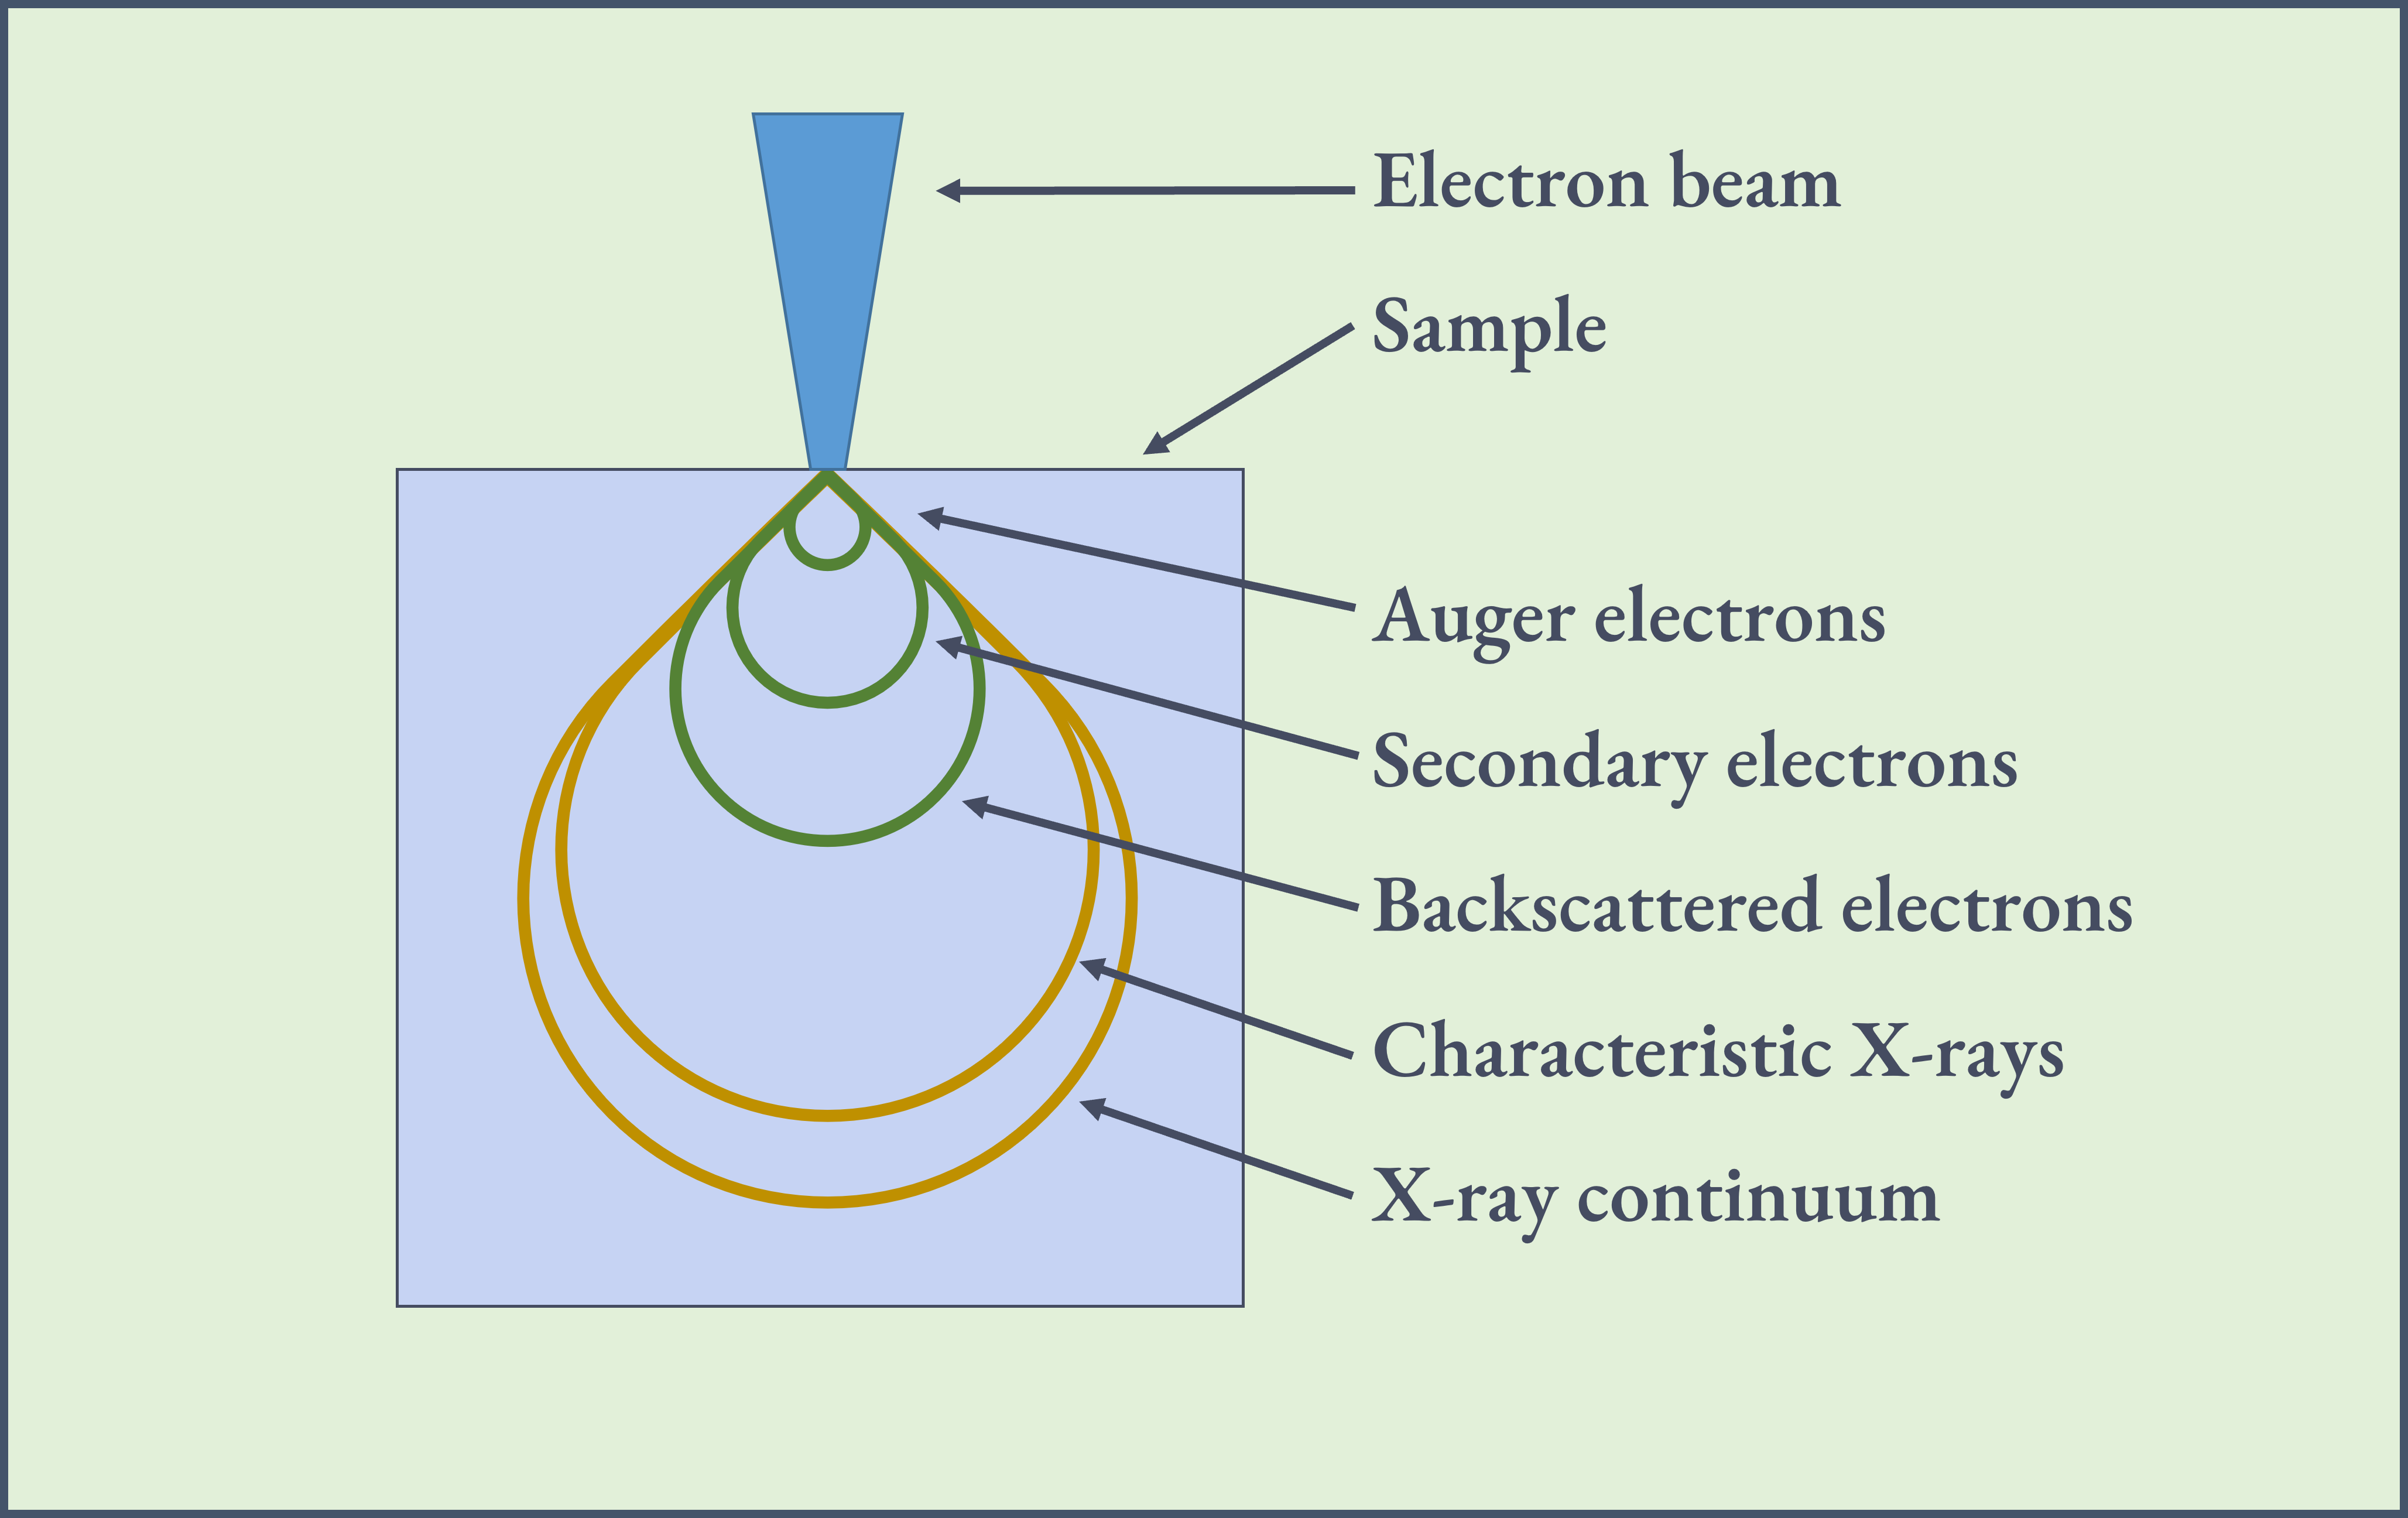
\includegraphics[width=0.8\linewidth]{figures/interaction_volume.png}
    \caption{
        Illustration of the interaction volume of the different signals.
        The signals are emitted in all directions, which is why the interaction volume is spherical.
        The blue signals are electrons and the orange signals are X-rays.
        The depths are not to scale.
    }
    \label{fig:interaction_volume}
\end{figure}


\ton{Do you want me to write about the different signals, ie. SE and BSE?}


% The parts in the SEM
An SEM consists of several parts, which are illustrated in \cref{fig:SEM_setup}.
The electron gun is the source of the electrons.
The condenser lens focuses the electrons to a small beam.
The two apertures sets the size of the beam, which is important since the electrons closest to the central axis of the beam have fewest aberrations.
The scanning coils are used to scan the beam over the sample in the raster fashion.
The objective lens focuses the beam to a small spot on the sample.
In general a smaller spot allows higher resolution, because the signal is recorded from a smaller area.
However, this effect is limited by several factors, such as the interaction volume.
The detectors are placed above the sample.

\ton{What more do you want me to write about the SEM?}

% figure/SEM_setup.png
\begin{figure}[ht]
    \centering
    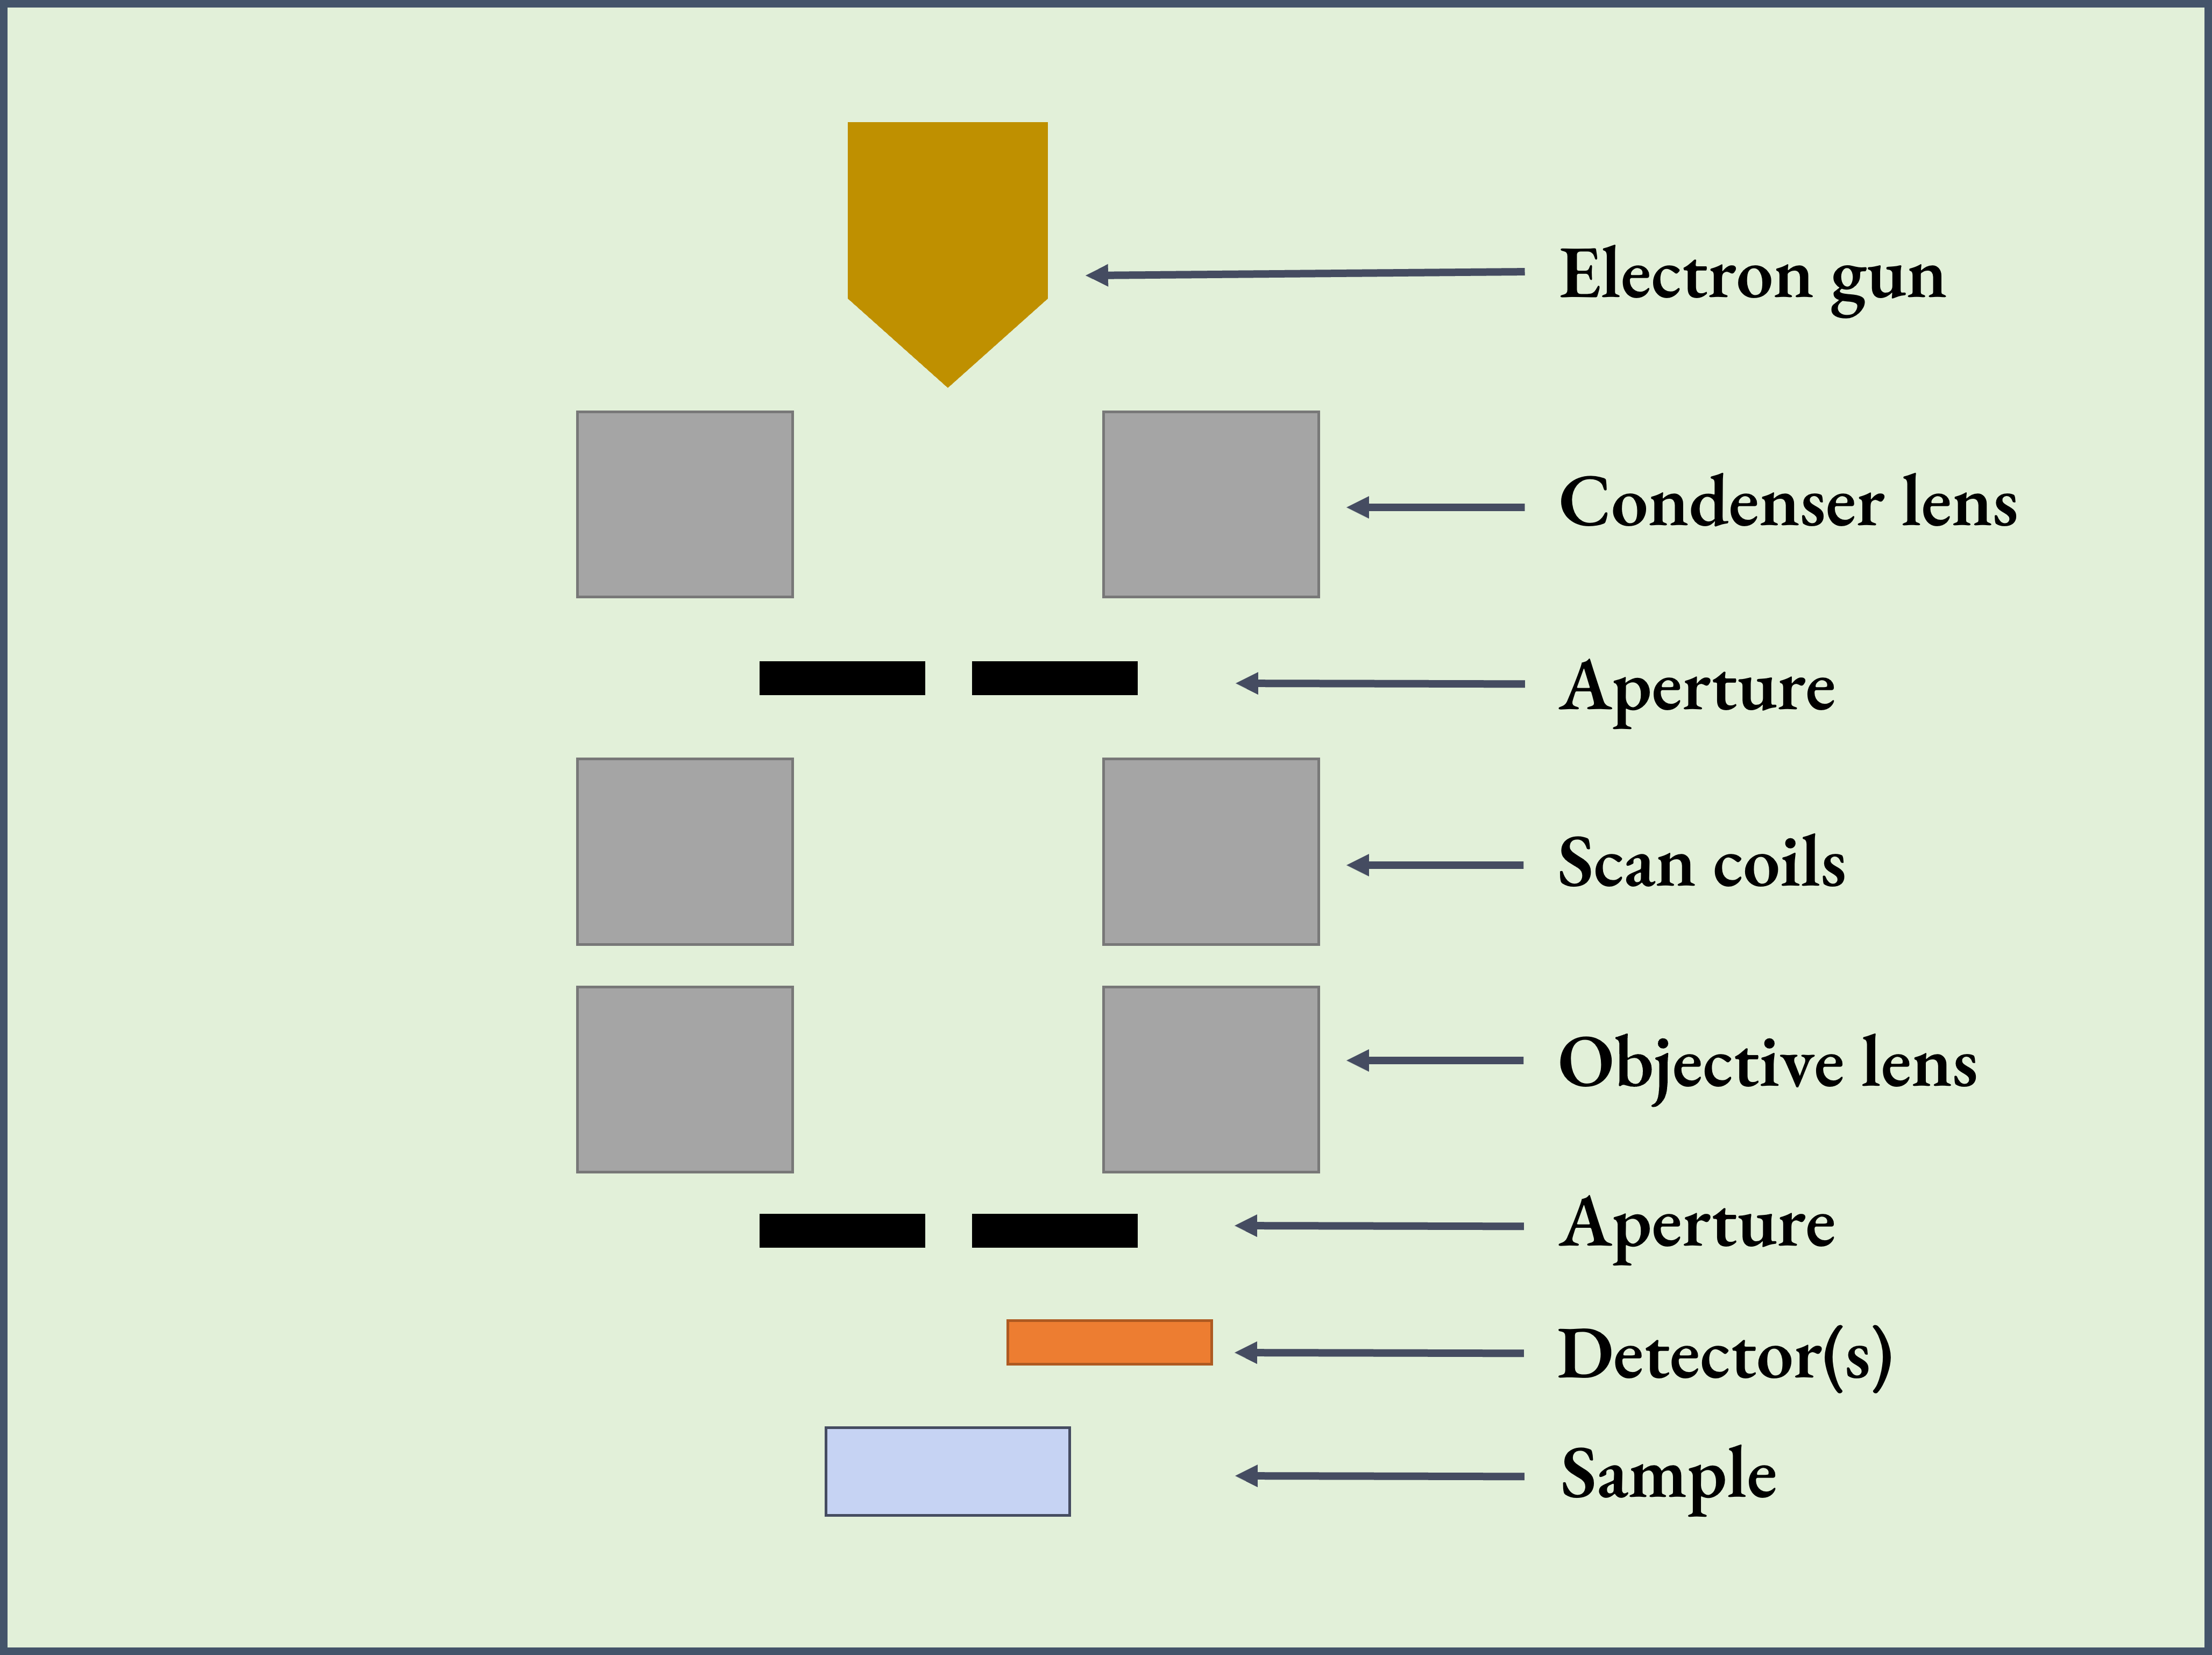
\includegraphics[width=0.8\linewidth]{figures/SEM_setup.png}
    \caption{
        Illustration of the parts in an SEM.
    }
    \label{fig:SEM_setup}
\end{figure}






\section{Quality control - detector characterization}
\label{theory:qc}

The aim of this work is to improve EDS bulk quantification, and one way to do this is to make the input parameters of the quantification more accurate and doing a health check on the detector.
Manufactors of EDS detectors like Oxford Instruments provide a guide for how to perform quality control on their detector, but these guides focus only on calibration of energy resolution and scale \cite{aztec_manual}.
The state of an EDS setup is characterized by more than its energy resolution and scale, and this section describes how to perform a health check on the detector.
Little literature is published on quality control programs for SEM EDS setups, but there are several papers on tests for TEM EDS.
% Mari: The tests are described by Watanabe in [30] and in the info-sheet by Ted Pella [33] which is based on the original work by R.F. Egerton and C.S. Cheng from 1994 [16].
% The complete test routine has several characteristics. Here only the most essential to this work are discussed, and an overview is found in Tab. 2.3.
One of the challenges in this work is to find the find the most relevant test characteristics, and what ranges of values are acceptable for a healthy detector.
Each test characteristics is described with what it is, how it is measured, and what values are acceptable.



\subsection{Duane-Hunt}
\label{theory:qc:duanehunt}
% put after calibration? It is done before in the code, but it is not a part of AZtec.

% What
Finding the real $E_0$.
Used to slice the spectrum at the correct energy.

% How
Linear regression of background.

% Acceptable values
$E_0$ should be within X\% of the specified acceleration voltage.
Large deviations implicate \dots

\subsection{Calibration of energy resolution}
\label{theory:qc:energyres}

% What
What is the energy resolution.
What is a good energy resolution.
Why Mn K$\alpha$?
Finding the calibrated energy resolution, Mn K$\alpha$.

% How
Measure the FWHM of a Mn K$\alpha$ peak if possible.
\brynjar{Implement check for Mn K$\alpha$ peak in the code.}
Else, use HS function for estimating a peak width at the Mn K$\alpha$ energy.
Alternatively, as Ted Pella suggests, use the FWHM of Ni K$\alpha$ peak and multiply by 0.926, which is based on data from multiple detectors.

% Acceptable values
The energy resolution should be close to what the manufacturer specifies.
HyperSpy defines a energy resolution below 110 eV as impossible \brynjar{Check the number and add reference to the code line}.
Large deviations implicate \dots


\subsection{Calibration of scale and offset}
\label{theory:qc:scaleoffset}
% scale and offset in one subsection?

% What
What is the scale and offset.
Typical values for the scale.

% How
Measure two far apart peaks and find their distance in the spectrum.
Or, use the HS function, which does \dots

% Acceptable values
Deviations should be \dots
Large deviations implicate \dots


\subsection{Calibrating peak positions}
\label{theory:qc:peakpositions}

% What
What is the peak position.
Also mention the peak width?
Why does it deviate from the theoretical value.
Figure of Mo K$\alpha$ peak which is not centered?
Why bigger changes at higher energies.

% How
Manual: add gaussians at the expected position and fit.
HS: adds gaussians at the expected position and fit with the centre as free parameter.

% Acceptable values
Deviations can be higher at higher energies, but should be \dots
Large deviations implicate \dots


% one section on the calculated value for each line of interest?
% Line           True E [keV]   Calib. E [keV] Area [counts]  Max (fit)      Sigma [keV]    FWHM [eV]      Fiori P_10/B

\subsection{Fiori peak to background ratio}
\label{theory:qc:fiori}


\subsection{Peak ratio}
\label{theory:qc:peakratio}
% contaminations, at least for TEM


\subsection{Peak shape}
\label{theory:qc:peakshape}
% The real lines are Lorentzians with width of 1-10 eV, but the peaks are wider due to electronic noise.
% Peaks are gaussians by electronic noise.
% a measure of the peak shape is the FWTM/FWHM


\subsection{Number of counts in peaks vs background}
\label{theory:qc:counts}

% Total counts, background counts.
% How to represent the measure better? Ratio, percentage, absolute value, etc.
% Fiori P/B is a measure already covered.

